\documentclass[11pt,a4paper]{article}
\usepackage{a4wide}
\usepackage[utf8]{inputenc}
\usepackage[T2A]{fontenc}
\usepackage{graphics,graphicx,epsfig}
\usepackage{amssymb,amsfonts,amsthm,amsmath,mathtext,cite,enumerate,float}
\usepackage[english,russian]{babel}
\usepackage[all]{xy}
\usepackage{morefloats}
\usepackage{pgf}
\usepackage[debug,outputdir={docgraphs/}]{dot2texi}
\usepackage{tikz}
\usepackage{scalefnt}
\usepackage{listings}
\usepackage{float}
\usepackage{verbatim}
\usepackage{placeins}
\usepackage{url}
\usepackage{babelbib}
\usepackage{pbox}
\usepackage{grffile}
\usepackage{color}
\usepackage{xfrac}
\usepackage{comment}
\usepackage{rotating}
\usepackage{cite}
\usepackage{sectsty}
\usepackage{caption}
\usepackage{subcaption}
\usetikzlibrary{shapes,arrows}
\usetikzlibrary{decorations.pathmorphing}

% Comment the following block when compiling this .tex with a saner compiler than texlive.
\makeatletter
\def\@settitle{\begin{center}%
    \baselineskip14\p@\relax
    \bfseries
    \@title
  \end{center}%
}

\renewcommand{\citedash}{]-[}
\renewcommand{\citepunct}{], [}

\renewcommand{\thesubfigure}{\asbuk{subfigure}}
\addto\captionsrussian{\renewcommand{\figurename}{Фиг.}}

\sectionfont{\centering\normalfont\small\MakeUppercase}

%\renewcommand{\section}{\@startsection {section}{1}%
%  \z@{.7\linespacing\@plus\linespacing}{.5\linespacing}%
%  {\normalfont}}
%\renewcommand{\section}{\@startsection {section}{1}
%  \z@{2.7ex \@plus 1ex}{1.0ex}%
%  {\normalfont}}
\makeatother

\theoremstyle{definition}
\newtheorem{algo}{Алгоритм}
\newtheorem{theorem}{Теорема}
\newtheorem{stat}{Утверждение}
\newtheorem{defin}{Определение}
\newtheorem{note}{Замечание}

\begin{document}

\begin{center}
  STABILITY OF NON-LINEAR REGRESSION MODELS WITH RESPECT TO VARIATIONS IN THE MEASURED DATA

  \bigskip
  G.~Rudoy.
\end{center}

\begin{abstract}
  A set of inductively generated non-linear regression models is considered to find an optimal
  one. Firstly, a previously suggested model generation method taking the complexity of the
  models into account is applied. Then, a new model selection criteria is proposed, called
  model stability, which shows the dependency of the inaccuracy in determining the coefficients
  of the generated models on the variation of the data in the learning set. This criteria
  is used directly to determine the inaccuracy of the model coefficients, which is of interest
  to the experts, as well as to select the optimal model amongst different ones generated
  using different algorithm hyperparameters.
  The data obtained during experiments on optical dispersion of transparent polymers is used
  to illustrate the method.

  \bigskip
  \textbf{Keywords}: \emph{symbolic regression, non-linear models, inductive generation,
	model stability, transparent polymers dispersion.}
\end{abstract}

\section*{Introduction}

Analysing the results of a physical experiment typically requires finding a functional
dependency between the measured data. It is also very desirable for the dependency to
be interpretable by an expert in the corresponding physical field. In many cases some
theoretical assumptions about the structure of the functional dependency are available,
or a choice should be made between different proposed models.

One of the methods allowing to find interpretable models is symbolic regression
\cite{davidson:2000:snrea,reference/ml/X10vc,StrijovW10,Strijov08InductMethods,Rudoy13},
which generates structurally complex non-linear models. Different models
can be compared by their respective errors on the measured data,
and the optimization of their numeric parameters is performed, for example, using
the Levenberg-Marquardt algorithm\cite{Marquardt1963Algorithm,more:78}.

On the other hand, during physical experiment analysis not only the model
parameters themselves are important for the expert, but the uncertainities in
determining their values resulting from the intrinsic measurement inaccuracies.
For the linear regression this problem is known to have a theoretical solution\cite{Vatunin05}
in the particular case of the independent variable measured exactly and the
dependent variable having the same Gaussian distribution of the error at all
measured points. More complex case of non-linear regression, including the case
of independent variables measured inexactly, as well as all points having
different error distributions, has not been considered as far as we know.

In this paper the non-linear symbolic regression method is applied to find
the dependency of the refraction index $n$ of a polymer as a function of the
wavelength $\lambda$ for those frequencies where the considered polymer is
transparent, including visible and near infrared light. The goal of the
experimenters was to, first, find the dispersion for each polymer, and then
derive the concentration of each polymer in their mixture, given that the
dispersion of the mixture of polymers is a weighted sum of their respective
dispersions. In other words, in case of two polymers, knowing the functions
$n_1(\lambda)$ and $n_2(\lambda)$, the mixture dispersion dependency $n(\lambda)$ 
should be measured and, since
$n(\lambda) = \alpha n_1(\lambda) + (1 - \alpha) n_2(\lambda)$, the concentration
of the first polymer $\alpha$ should be derived.

The refraction indexes for the transparent polymers of a similar chemical
composition differ only slightly. Thus, the uncertainity in determining the
$n(\lambda)$ function coefficients and its dependency on the inaccuracies of measurements
of the wavelength $\lambda$ and refraction index $n$ must be considered.
This dependency is also important because it defines the requirements for the
precision of the devices and, consecutively, it largely
affects the cost and duration of the experiment.

Typically broad spectrum sources are used in refractometers, and the
inaccuracy in extracting a single wavelength is defined by the hardware function
of the monochromator being used and is thorougly considered, for example, in
\cite{Malishev79,Zaidel72}. In most cases the inaccuracy of $\lambda$ can be
computed as well as determined experimentally using narrow light sources like
lasers, known atomic transitions like the mercury triplet or sodium dublet.
Typical relative wavelength measurement inaccuracy is around $0.03 \div 0.5\%$,
thus absolute inaccuracy depends on the wavelength itself. Inaccuracy of
the refraction index $n$ depends on the measurement method and, for example,
in case of using the total internal refraction angle, is defined by the degree
of non-parallelism of the light beams used, the inaccuracy in angle measurement
and so on. The inaccuracy ranges from $(1 \div 2) \cdot 10^{-5}$ for high-class
devices to $(1 \div 10) \cdot 10^{-4}$ for simpler devices. Thus, it is important
for this paper that the inaccuracies can be considered to be known and perhaps
different for each data point.

In this paper the dependency of the refraction index of the wavelength is used
to illustrate the model generation algorithm proposed in \cite{Rudoy13}.
Its results are compared with the SVM regression. Moreover, the impact of the
complexity penalty on the quality and complexity of the generated models
is investigated. The problem of determining the model coefficients stability
in the general case of multivariate models is formally stated, a method for evaluating
solution stability is proposed, and the dependency of these characteristics of
the model hyperparameters is studied for the given case of determining the dispersion
of transparent polymers.

In the first part of this paper the dispersion problem is formally stated, and the
stability criteria is proposed. In the second part the algorithm proposed in\cite{Rudoy13},
used to generate the regression model, is briefly described. In the third part a
numeric method for stability estimation is proposed. In the fourth part the results
of the computational experiment are shown. In the experiment two polymers are considered,
for each of them 17 data points are given, corresponding to the refraction index at
different wavelengths.

\section{Постановка задачи}

\paragraph{Задача регрессии.}
Дана выборка $D$ из $\ell$ результатов измерений коэффициента
преломления для некоторого полимера:
$D = \{ \lambda_i, n_i \mid i \in \{ 1, \dots, \ell \} \}$, где $\lambda_i$~--- длина волны,
а $n_i$~--- измеренный коэффициент преломления в $i$-ом измерении.

Требуется найти функцию $\hat{f} = \hat{f}(\lambda)$, минимизирующую стандартный
функционал потерь в предположении о нормальности случайной ошибки эксперимента:
\begin{equation}
  S(f, D) = \sum_{i = 1}^\ell (f(\lambda_i) - n_i)^2 \rightarrow \min_{f \in \mathcal{F}},
  \label{eq:s}
\end{equation}
где $D = \{ \lambda_i, n_i\}$, а $\mathcal{F}$~---
некоторое множество суперпозиций, из которого выбирается оптимальная.

Иными словами,
\begin{equation}
  \hat{f}(\lambda) = \hat{f}_D(\lambda) = \mathop{\arg \min}\limits_{f \in \mathcal{F}} S(f, D).
  \label{eq:fhat}
\end{equation}

\paragraph{Задача оценки устойчивости.}
Введем в общем виде понятие устойчивости суперпозиции $f$, характеризующей
поведение коэффициентов суперпозиции $\hat{f}$ при небольшом случайном
изменении исходной обучающей выборки
$D = \{ \mathbf{x}_i, y_i \}$,
где $\mathbf{x}_i$~--- исходное (полученное в ходе эксперимента)
признаковое описание $i$-го объекта, а $y_i$~--- соответствующее экспериментально
измеренное значение функции, которую требуется восстановить.

Функционал потерь \eqref{eq:s} в этом случае выглядит следующим образом: 
\begin{equation}
  S(f, D) = \sum_{i = 1}^\ell (f(\mathbf{x}_i) - y_i)^2 \rightarrow \min_{f \in \mathcal{F}}.
  \label{eq:s_common}
\end{equation}

Условимся также обозначать матрицу плана $X = \| x_{ij} \|$, строками которой
являются признаковые описания объектов выборки $D$. Иными словами, $x_{ij}$
обозначает $j$-ую компоненту признакового описания $i$-го объекта.

Рассмотрим вектор параметров
$\boldsymbol{\omega}_f = \{ \omega_i^f \mid i \in \{ 1, \dots, l_f \} \}$
некоторой суперпозиции $f$: $f(\mathbf{x}) = f(\mathbf{x}, \boldsymbol{\omega}_f)$.
Пусть для некоторой выборки $D = \{ \mathbf{x}_i, y_i \}$ и функции
$f$ вектор параметров $\hat{\boldsymbol{\omega}}_f(D)$ минимизирует
функционал \eqref{eq:s_common} с суперпозицией $f$, имеющей фиксированную
структуру:
\[
  \hat{\boldsymbol{\omega}}_f(D) = \mathop{\arg \min}\limits_{\boldsymbol{\omega}_f} S(f, D).
\]

Пусть также дана матрица стандартных отклонений
независимых переменных $\Sigma^{\mathbf{x}} = \| \sigma^{\mathbf{x}}_{ij} \|$,
где $\sigma^{\mathbf{x}}_{ij}$ характеризует стандартное отклонение $j$-ой
компоненты признакового описания $\mathbf{x}_i$ $i$-го объекта обучающей выборки,
и вектор стандартных отклонений $\boldsymbol{\sigma}^y$, где $\sigma^y_i$
характеризует стандартное отклонение зависимой переменной, соответствующей
$i$-му объекту.
Рассмотрим выборку $\acute{D}$, полученную из исходной выборки $D$
добавлением к каждой компоненте реализаций нормально распределенных
случайных величин с нулевым матожиданием и соответствующей
$\Sigma^{\mathbf{x}}$ и $\boldsymbol{\sigma}^y$ дисперсией:
\begin{equation}
  \acute{D}(\Sigma^{\mathbf{x}}, \boldsymbol{\sigma}^y) = \{ \mathbf{x}_i + \boldsymbol{\xi}^{\mathbf{x}}_i, y_i + \xi^y_i \mid i \in 1, \dots, \ell; \boldsymbol{\xi}^{\mathbf{x}}_i \sim \mathcal{N}(0; \boldsymbol{\sigma}^{\mathbf{x}}_{i \cdot}); \xi^y_i \sim \mathcal{N}(0; \sigma^y_i) \}.
  \label{eq:d_acute}
\end{equation}

Для этой выборки $\acute{D}$ найдем оптимальный вектор $\hat{\boldsymbol{\omega}}_f (\acute{D} (\Sigma^{\mathbf{x}}, \boldsymbol{\sigma}_y))$
параметров суперпозиции $f$, минимизирующий функционал \eqref{eq:s}:
\begin{equation}
  \hat{\boldsymbol{\omega}}_f (\acute{D} (\Sigma^{\mathbf{x}}, \boldsymbol{\sigma}_y)) = \mathop{\arg \min}\limits_{\boldsymbol{\omega}_{f_D} \in R^{\mid \hat{\boldsymbol{\omega}}_f \mid}} S (f_D (\cdot, \boldsymbol{\omega}_{f_D}), \acute{D} (\Sigma^{\mathbf{x}}, \boldsymbol{\sigma}_y)).
  \label{eq:hat_omega}
\end{equation}
Понятно, что $\hat{\boldsymbol{\omega}}_f (\acute{D} (\Sigma^{\mathbf{x}}, \boldsymbol{\sigma}_y))$~---
векторная случайная величина, и, следовательно,
\[
  \Delta\hat{\boldsymbol{\omega}}_f(\acute{D} (\Sigma^{\mathbf{x}}, \boldsymbol{\sigma}_y) ) = \hat{\boldsymbol{\omega}}_f(D) - \hat{\boldsymbol{\omega}}_f (\acute{D} (\Sigma^{\mathbf{x}}, \boldsymbol{\sigma}_y))
\]
также векторная случайная величина.

Пусть дано множество $\acute{\mathcal{D}}_N$ из $N$ таких выборок, где каждая выборка
соответствует отдельным реализациям случайных величин из \eqref{eq:d_acute}:
\[
  \acute{\mathcal{D}}_N (\Sigma^{\mathbf{x}}, \boldsymbol{\sigma}_y) = \{ \acute{D}_1 (\Sigma^{\mathbf{x}}, \boldsymbol{\sigma}_y), \dots, \acute{D}_N (\Sigma^{\mathbf{x}}, \boldsymbol{\sigma}_y) \},
\]
и пусть $\overline{\sigma}_i$~--- эмпирическое стандартное отклонение $i$-ой компоненты
векторной случайной величины
$\Delta\hat{\boldsymbol{\omega}}_f(\acute{D} (\Sigma^{\mathbf{x}}, \boldsymbol{\sigma}_y) )$
на множестве $\acute{\mathcal{D}}_N (\Sigma^{\mathbf{x}}, \boldsymbol{\sigma}_y)$.
\begin{defin}
\emph{Относительной устойчивостью} (или просто \emph{устойчивостью}) параметра
$\omega_i$ относительно $\acute{\mathcal{D}}_N (\Sigma^{\mathbf{x}}, \boldsymbol{\sigma}_y)$
при исходной обучающей выборке $D$ будем называть следующий вектор
из $| \mathbf{x} | + 1$ компонент:
\begin{equation}
  \mathbf{T}^N_f(i) = \Big\{ \frac{\frac{\overline{\sigma}_i}{\hat{\omega}_i}}{r(\boldsymbol{\sigma}^\mathbf{x}_{\cdot 1}, \mathbf{x}_{\cdot 1})}, \dots, \frac{\frac{\overline{\sigma}_i}{\hat{\omega}_i}}{r(\boldsymbol{\sigma}^\mathbf{x}_{\cdot |\mathbf{x}|}, \mathbf{x}_{\cdot |\mathbf{x}|})}, \frac{\frac{\overline{\sigma}_i}{\hat{\omega}_i}}{r(\boldsymbol{\sigma}^y, \mathbf{y})} \Big\},
  \label{eq:t_rel}
\end{equation}
где $r(\boldsymbol{\alpha}, \mathbf{a}) = r(\frac{\alpha_1}{a_1}, \dots, \frac{\alpha_{|\boldsymbol{\alpha}|}}{a_{|\mathbf{a}|}})$~---
функция, переводящая вектор, составленный из отношений соответствующих компонент векторов $\boldsymbol{\alpha}$ и $\mathbf{a}$, в скаляр.
\end{defin}

Функция $r$ позволяет сопоставить, вообще говоря, различным отношениям стандартного
отклонения зависимой переменной $y_i$ $i$-го объекта обучающей выборки и самого значения $y_i$
единственное число (аналогично и для $x_i$-й независимой переменной и ее стандартного отклонения).
Примерами такой функции могут являться среднее арифметическое
всех отношений или максимальное значение отношения, а конкретная функция выбирается
экспертом в зависимости от физического смысла задачи.
В настоящей работе предлагается выбирать значения стандартных отклонений так, чтобы
все значения соответствующих переменных были равны, поэтому функция $r$ может выбирать
любой из своих аргументов.

Каждый компонент вектора $\mathbf{T}^N_f(i)$ показывает, как относится стандартное отклонение
параметра $\hat{\omega}_i$, нормированное на значение этого параметра, к характерному стандартному
отклонению соответствующего элемента признакового описания, нормированного на значение этого
элемента. Например, если это отношение больше единицы, то погрешности определения коэффициента
растут быстрее погрешностей измерения параметра.

В частности, в искомой задаче восстановления дисперсионной зависимости с учетом неизменной
относительной ошибки эксперимента:
\[
  \mathbf{T}_f(i) = \Big\{ \frac{\frac{\overline{\sigma}_i}{\hat{\omega}_i}}{\frac{\sigma_n}{n}}, \frac{\frac{\overline{\sigma}_i}{\hat{\omega}_i}}{\frac{\sigma_{\lambda}}{\lambda}} \Big\}.
\]

Матрицу, столбцами которой являются векторы $\mathbf{T}_f(i) \mid i \in \{ 1, \dots, l_f \}$,
будем называть устойчивостью функции $f$ и обозначать $\mathbb{T}_f$.

Требуется исследовать зависимость устойчивости $\mathbb{T}_{\hat{f}}$ относительно
$\sigma_n$ и $\sigma_{\lambda}$.

\section{Алгоритм индуктивного порождения суперпозиций}

Опишем предложенный в \cite{Rudoy13} алгоритм.

Пусть задано некоторое множество $G = \{ g_1, \dots, g_k \}$ 
порождающих функций. Набор суперпозиций $\mathcal{F} = \{ f \}$
инициализируется случайными суперпозициями функций $g \in G$. Суперпозиции из
$\mathcal{F}$ содержат как свободные переменные, соответствующие
компонентам вектора-описания объектов из генеральной совокупности, так и
константы, которые оптимизируются на каждом шаге алгоритмом Левенберга-Марквардта
согласно введенному функционалу потерь \eqref{eq:s}. Также на каждой итерации
над суперпозициями выполняется набор модифицирующих операций с целью улучшения
качества $Q_f$ суперпозиций.

Качество $Q_f$ суперпозиции $f$ вычисляется по совокупности точности приближения
экспериментальных данных и структурной сложности суперпозиции по следующей формуле:
\begin{equation}
  Q_f = \frac{1}{1 + S(f)} \left(\alpha + \frac{1 - \alpha}{1 + \text{exp} (C_f - \tau)}\right),
  \label{eq:s_f}
\end{equation}
где:
\begin{itemize}
  \item[] $S(f)$~--- значение функционала потерь \eqref{eq:s} на данной выборке $D$;
  \item[] $C_f$~--- сложность суперпозиции, соответствующая количеству элементарных
	функций, свободных переменных и констант;
  \item[] $\alpha$~--- $0 \ll \alpha < 1$, характеризует влияние штрафа за сложность
	на качество суперпозиции (большие значения $\alpha$ отдают предпочтение более
	точным моделям, а меньшие~--- более простым);
  \item[] $\tau$~--- коэффициент, характеризующий желаемую сложность модели.
\end{itemize}

Второй множитель в \eqref{eq:s_f} выполняет роль штрафа за слишком
большую сложность суперпозиции, что подавляет эффект переобучения и позволяет
получать более простые суперпозиции ценой большей ошибки на обучающих данных
при большей обобщающей способности.

Отметим, что параметры $\alpha$ и $\tau$ выбираются экспертом.

Таким образом, исходная задача минимизации функционала \eqref{eq:s} заменяется
на задачу минимизации функционала \eqref{eq:s_f}:
\begin{equation}
  Q_f = \frac{1}{1 + S(f)} \left(\alpha + \frac{1 - \alpha}{1 + \text{exp} (C_f - \tau)}\right) \rightarrow \min_{f \in \mathcal{F}}.
  \label{eq:s_f_min}
\end{equation}

\section{Метод исследования стабильности решения}

Для оценки устойчивости $\mathbb{T}_{\hat{f}}$ решения $\hat{f}$ задачи
\eqref{eq:s_f}, как предложено выше, фиксируется структурный вид суперпозиции
$\hat{f}$ и исследуется зависимость стандартного отклонения ее коэффициентов
как функция стандартного отклонения нормально распределенной случайной добавки
в исходных данных.

Иными словами, выбираются значения $\sigma_{\lambda}$ и $\sigma_n$, затем для этих
значений генерируется выборка $\acute{D}(\sigma_n, \sigma_{\lambda})$ согласно
\eqref{eq:d_acute}. Для этой выборки вычисляются значения коэффициентов суперпозиции
$\hat{f}$, минимизирующие функционал \eqref{eq:s} согласно \eqref{eq:hat_omega},
методом Левенберга-Марквардта.

Данная процедура для фиксированной пары $\sigma_{\lambda}$ и $\sigma_n$ повторяется
до достижения некоторого критерия останова (например, по количеству итераций),
после которого и рассчитывается $\mathbb{T}_{\hat{f}}$.

Повторяя описанные выше шаги для различных $\sigma_{\lambda}$ и $\sigma_n$, можно
оценить зависимость стандартного отклонения коэффициентов суперпозиции от
стандартного отклонения шума.

Из физических соображений ясно, что гладкая зависимость означает устойчивое в
физическом смысле решение, тогда как отклонения от гладкости означают
ту или иную ошибку в суперпозиции и могут являться свидетельством переобучения:
чем меньше коэффициенты зависят от случайных шумов в данных, тем больше обобщающая
способность.

Кроме того, сравнение различных суперпозиций может также производиться по
критерию устойчивости в дополнение к сравнению по сложности и по значению
функционала \eqref{eq:s}. В ряде практических приложений критерий устойчивости
может иметь приоритетное значение.

\section{Вычислительный эксперимент}

В вычислительном эксперименте используются данные, полученные в ходе
изучения возможности определения состава смеси прозрачных
полимеров по суммарной дисперсионной зависимости, если известна экспериментальная
зависимость дисперсии для каждого конкретного полимера. Рассматривается два
полимера, для каждого из которых имеется 17 экспериментальных точек,
соответствующих коэффициенту преломления при разных значениях длины волны.
Значения приведены в таблице \ref{tabl:source_data}.

\begin{table}[h]
  \footnotesize
  \caption{Экспериментальные значения коэффициентов преломления.}
  \centering
  \begin{tabular}{r | r | r}
	$\lambda$, нм	& Полимер 1 & Полимер 2 \\ \hline
	435.8 & 1.36852 & 1.35715 \\
	447.1 & 1.36745 & 1.35625 \\
	471.3 & 1.36543 & 1.35449 \\
	486.1 & 1.36446 & 1.35349 \\
	501.6 & 1.36347 & 1.35275 \\
	546.1 & 1.36126 & 1.35083 \\
	577.0 & 1.3599 & 1.34968 \\
	587.6 & 1.3597 & 1.34946 \\
	589.3 & 1.35952 & 1.34938 \\
	656.3 & 1.35767 & 1.34768 \\
	667.8 & 1.35743 & 1.34740 \\
	706.5 & 1.35652 & 1.34664 \\
	750 & 1.35587 & 1.34607 \\
	800 & 1.35504 & 1.34544 \\
	850 & 1.3544 & 1.34487 \\
	900 & 1.35403 & 1.34437 \\
	950 & 1.35364 & 1.34407 \\
  \end{tabular}
  \label{tabl:source_data}
\end{table}

Предполагается, что дисперсионные свойства полимеров описываются одной и той
же функциональной зависимостью, так как подчиняются одним и тем же физическим
закономерностям. Поэтому сначала получена суперпозиция $\hat{f}$,
минимизирующая \eqref{eq:s_f} для первого полимера, а затем для каждого
из полимеров находятся соответствующие векторы параметров
$\hat{\boldsymbol{\omega}}_{\hat{f}}$ и оценивается устойчивость полученного решения.

Разделение на обучающую и контрольную выборку не производилось, однако переобучения
удается избежать и без такого разделения, опираясь целиком на штраф за сложность.

Из физических соображений следует \cite{Serova11}, что зависимость коэффициента
преломления $n$ от длины волны $\lambda$ должна выражаться суммой
четных степеней длины волны, поэтому множество элементарных функций состоит из
стандартных операций сложения и умножения:
\[
  g_1(x_1, x_2) = x_1 + x_2,
\]
\[
  g_2(x_1, x_2) = x_1 x_2,
\]
а также из функции
\[
  g_3(\lambda, p) = \frac{1}{\lambda^{2p}}.
\]

В ходе вычислительного эксперимента константы, меньшие $10^{-7}$,
заменялись на $0$.

В результате применения описанного выше алгоритма со значениями
$\alpha = 0.05$, $\tau = 10$ получена следующая суперпозиция
(константы округлены до пятой значащей цифры):
\begin{equation}
  f(\lambda) = 1.3495 + \frac{3.5465 \cdot 10^3}{\lambda^2} + \frac{2.023 \cdot 10^3}{\lambda^4},
  \label{eq:res_0}
\end{equation}
со сложностью $13$, среднеквадратичной ошибкой $2.4 \cdot 10^{-8}$ и значением $Q_f \approx 0.095$.
Длины волн выражаются в нанометрах.

Отметим, что обычно в приложениях учитывают только квадратичный член, а более
высокими степенями пренебрегают. Величина поправки, вносимой в результирующее значение
суперпозиции последним слагаемым, указывает на полное согласие полученных результатов
с принятой практикой.

\paragraph{Влияние штрафа за сложность.}

Исследуем, как влияет добавление нечетных степеней на результат решения задачи \eqref{eq:s_f_min},
заменив функцию $g_3$ в порождающем наборе на
\[
  g_3(\lambda, p) = \frac{1}{\lambda^p}.
\]

Следует отметить, что при тех же $\alpha = 0.05$ и $\tau = 10$ результирующей функцией остается
\eqref{eq:res_0}.

Увеличим $\tau$ до 30. Получим следующую формулу (константы округлены до третьей значащей цифры):
\begin{equation}
  n(\lambda) = 1.34 + \frac{11.6}{\lambda} + \frac{17.37}{\lambda^2} + \frac{0.0866}{\lambda^3} + \frac{2.95 \cdot 10^{-4}}{\lambda^4} + \frac{8.54 \cdot 10^{-7}}{\lambda^5},
  \label{eq:res_incorrect}
\end{equation}
сложность которой составляет $31$, и для которой среднеквадратичная ошибка
на выборке составляет $\approx 3.9 \cdot 10^{-9}$,
а значение $Q_f \approx 0.31$.

Иными словами, при большей желаемой сложности,
регулируемой параметром $\tau$, выигрывает более сложная (а в данном случае и
физически некорректная) модель, которая лучше описывает экспериментальные данные.

Как и следовало ожидать, чрезмерное увеличение $\tau$ ведет к переобучению.

\paragraph{SVM.}

В качестве базового алгоритма используется SVM-регрессия с RBF-ядром \cite{Vapnik79}.
Параметр $\gamma$ ядра подбирался по методу скользящего контроля, наилучшим результатом является
комбинация из $15$ опорных векторов c $\gamma \approx 2 \cdot 10^{-6}$, при этом
среднеквадратичная ошибка при кросс-валидации с тестовой выборкой, содержащей по 2
объекта, составляет $8.96 \cdot 10^{-8}$. Однако, проинтерпретировать полученную
решающую функцию не представляется возможным.

\paragraph{Исследование стабильности решения.}

Для оценки стабильности решения фиксировалась формула \eqref{eq:res_0} в виде
\[
  f(\lambda) = \omega_1 + \frac{\omega_2}{\lambda^2} + \frac{\omega_3}{\lambda^4},
\]
и исследовалась зависимость стандартного отклонения ее коэффициентов $\omega_1$,
$\omega_2$ и $\omega_3$ от стандартного отклонения
нормально распределенного случайного шума в исходных данных описанным выше методом.
Критерием останова в нем являлось достижение 10000 итераций для каждой пары
$(\sigma_{\lambda}, \sigma_n)$.

В таблице \ref{tabl:res_even} представлены
поверхности уровня дисперсии для первого, второго и третьего коэффициентов каждого из полимеров
соответственно.

\begin{table}[h]
  \centering
  \footnotesize
  \caption{Поверхности дисперсии для формулы \eqref{eq:res_0}.}
  \begin{tabular}{l | c c c}
	  & $\omega_1$ & $\omega_2$ & $\omega_3$ \\ \hline
	\begin{rotate}{90}Полимер 1\end{rotate} &	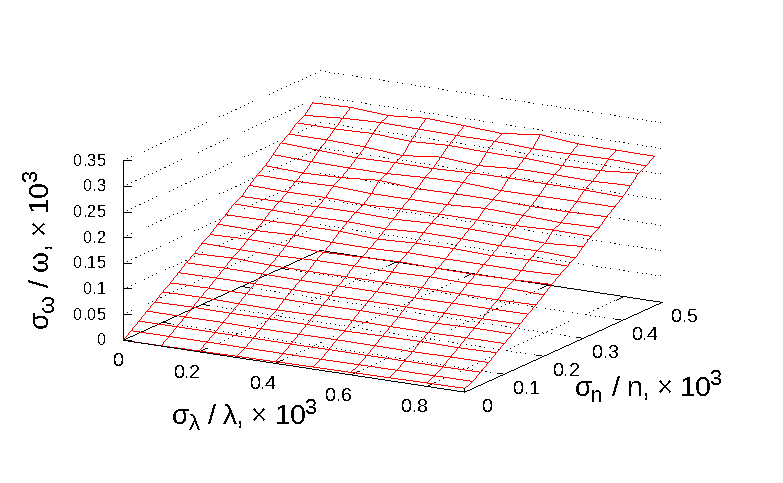
\includegraphics[scale=0.4]{figs/even/p1.txt_coeff0.dat.eps} & 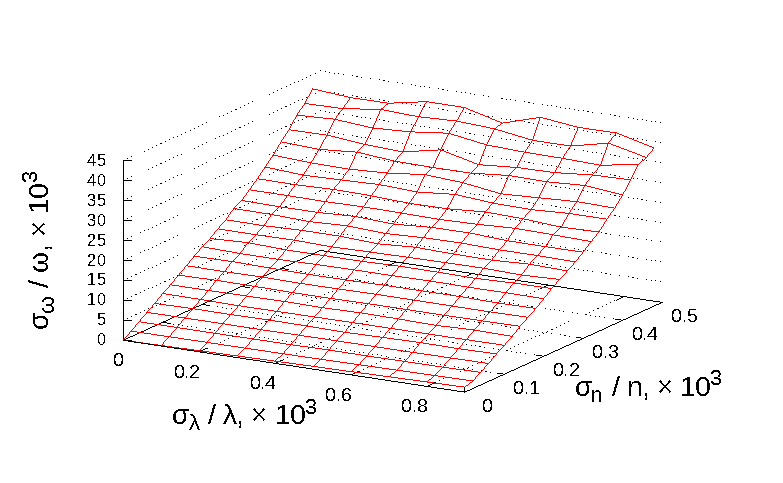
\includegraphics[scale=0.4]{figs/even/p1.txt_coeff1.dat.eps} & 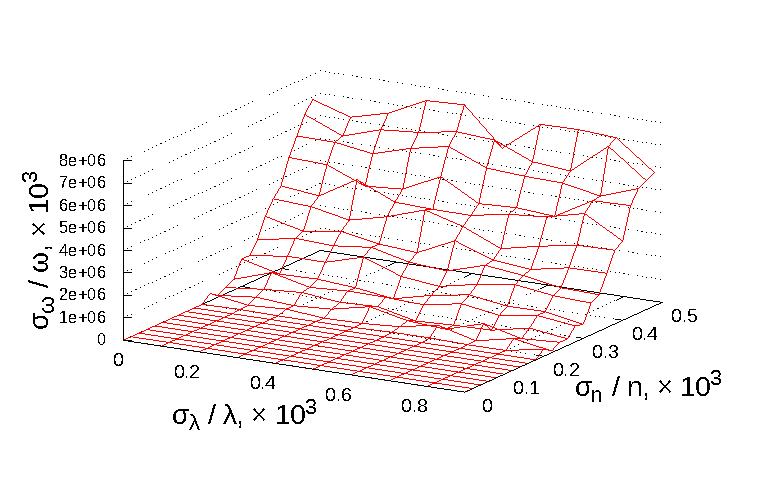
\includegraphics[scale=0.4]{figs/even/p1.txt_coeff2.dat.eps} \\
	\begin{rotate}{90}Полимер 2\end{rotate} &	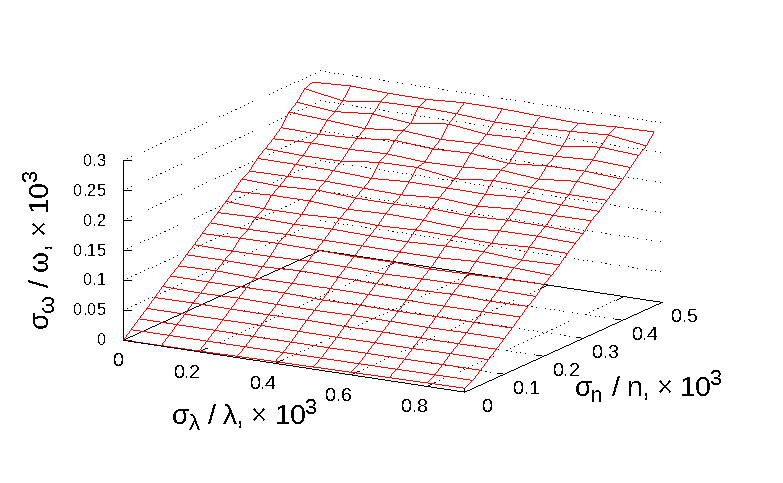
\includegraphics[scale=0.4]{figs/even/p2.txt_coeff0.dat.eps} & 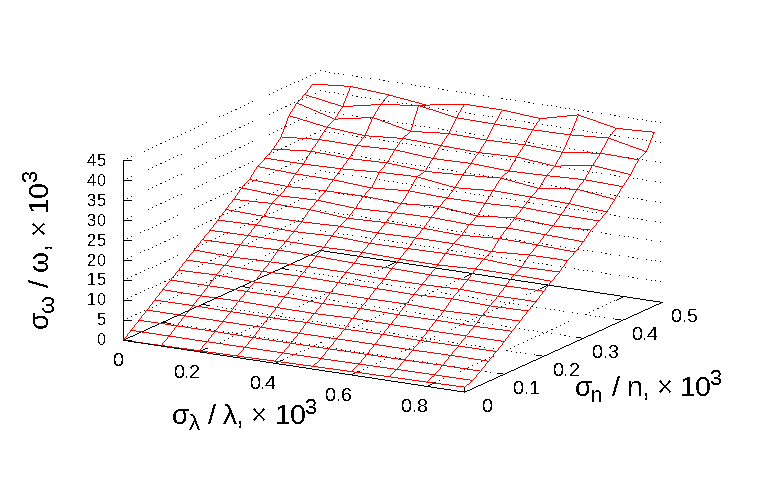
\includegraphics[scale=0.4]{figs/even/p2.txt_coeff1.dat.eps} & 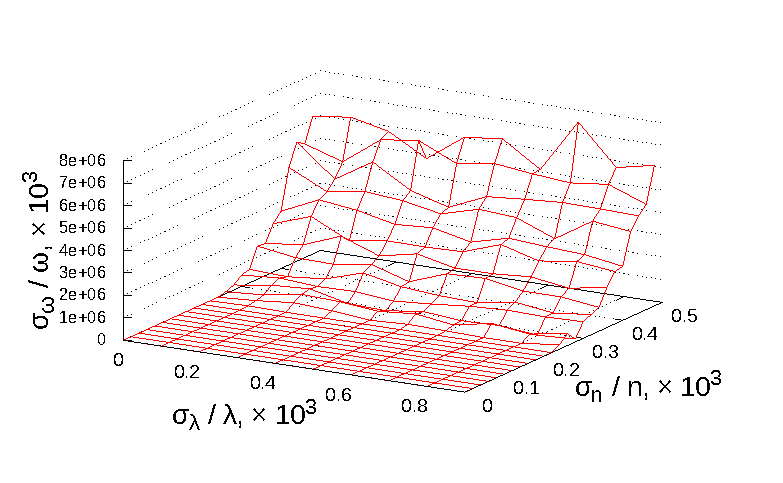
\includegraphics[scale=0.4]{figs/even/p2.txt_coeff2.dat.eps}
  \end{tabular}
  \label{tabl:res_even}
\end{table}

\begin{table}[h]
  \centering
  \footnotesize
  \caption{Значения коэффициентов для формулы \eqref{eq:res_0} и их относительная разность.}
  \begin{tabular}{l | c | c | c | c}
				& $\omega_1$				& $\omega_2$				& $\omega_3$				& MSE	\\ \hline
    Полимер 1	& 1.34946				& 3558.95				& 1924.33				& $2.2 \cdot 10^{-8}$		\\
    Полимер 2	& 1.34047				& 3118.84				& 1578.59				& $1.4 \cdot 10^{-8}$		\\
	Разность		& $6.71 \cdot 10^{-3}$	& $1.41 \cdot 10^{-1}$	& $2.2 \cdot 10^{-1}$	&	\\
  \end{tabular}
  \label{tabl:res_even_coeffs}
\end{table}

\begin{table}[h]
  \centering
  \footnotesize
  \caption{Значения стандартного отклонения для коэффициентов формулы \eqref{eq:res_0} для первого полимера в зависимости от относительных дисперсий.}
  \begin{tabular}{l | c | c | c}
	$\omega_i$	& $\frac{\sigma_{\lambda}}{\lambda} = 2 \cdot 10^{-4}; \frac{\sigma_n}{n} = 2 \cdot 10^{-5}$	& $ \frac{\sigma_{\lambda}}{\lambda} = 6 \cdot 10^{-4}; \frac{\sigma_n}{n} = 6 \cdot 10^{-5} $	& $ \frac{\sigma_{\lambda}}{\lambda} = 9 \cdot 10^{-4}; \frac{\sigma_n}{n} = 2 \cdot 10^{-4} $ \\ \hline
	1		& $1.22 \cdot 10^{-5}$																			& $ 3.59 \cdot 10^{-5} $																		& $ 1.19 \cdot 10^{-4} $		\\
	2		& $1.48 \cdot 10^{-3}$																			& $ 4.38 \cdot 10^{-3} $																		& $ 1.44 \cdot 10^{-2} $		\\
  \end{tabular}
  \label{tabl:res_even_stddev}
\end{table}

Из графиков видно, что от шума, накладываемого на значения длины волны, дисперсия значений
первого и второго коэффициентов практически не зависит в достаточно широком диапазоне точности
определения длины волны, представляющем практический интерес. В то же время дисперсия значений
первого коэффициента зависит от дисперсии шума коэффициента преломления практически линейно,
тогда как для второго коэффициента после некоторого характерного значения зависимость становится слабой.

Физическая интерпретация этих результатов~--- при построении прибора для измерения дисперсии
такого типа полимеров в их полосе прозрачности значительное внимание следует уделять точности измерения коэффициента преломления,
тогда как измерения длины волны могут быть неточны вплоть до нескольких нанометров. Кроме того,
предложенный метод прямо указывает, на каких интервалах шума каким будет выигрыш в точности
определения параметров регрессионной модели в зависимости от увеличения точности измерений.

Принципиально важно, что значения стандартного отклонения параметров регрессионной
модели существенно меньше разности между самими значениями этих параметров по порядку величины
(см. таблицы \ref{tabl:res_even_coeffs} и \ref{tabl:res_even_stddev}), что означает, в частности,
что полимеры могут быть различены даже не очень точным рефрактометром.

\paragraph{Стабильность некорректного решения.}

Аналогично исследуем стабильность решения \eqref{eq:res_incorrect}. Приведем только графики
зависимости первых трех коэффициентов, см. таблицу \ref{tabl:res_incorrect}.

\begin{table}[h]
  \centering
  \footnotesize
  \caption{Поверхности дисперсии для формулы \eqref{eq:res_incorrect}.}
  \begin{tabular}{l | c c c}
	  & $\omega_1$ & $\omega_2$ & $\omega_3$ \\ \hline
	\begin{rotate}{90}Полимер 1\end{rotate} &	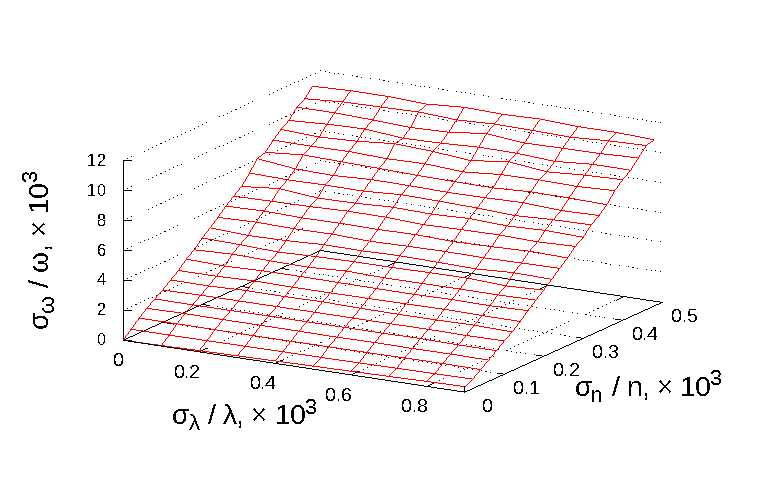
\includegraphics[scale=0.4]{figs/all/p1.txt_coeff0.dat.eps} & 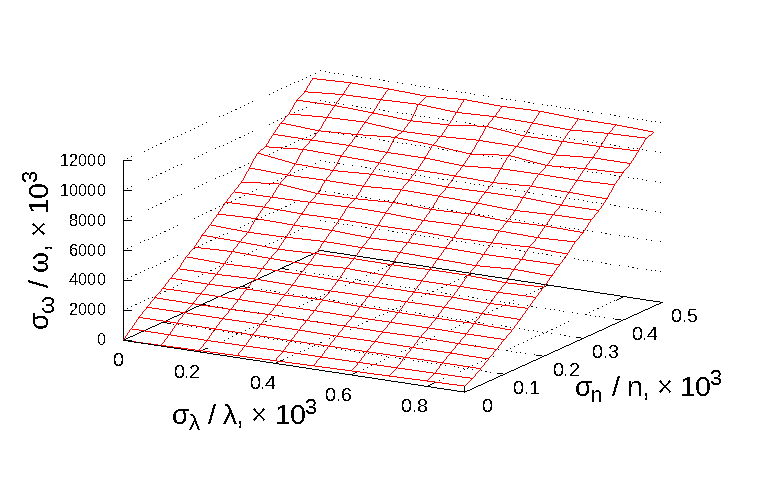
\includegraphics[scale=0.4]{figs/all/p1.txt_coeff1.dat.eps} & 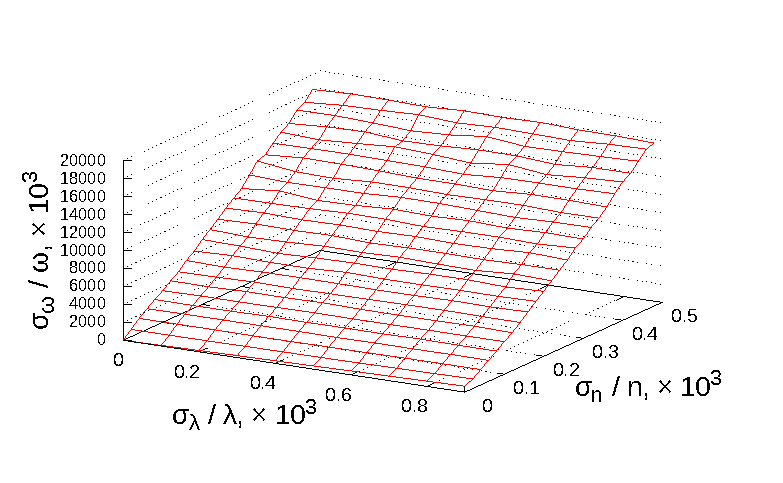
\includegraphics[scale=0.4]{figs/all/p1.txt_coeff2.dat.eps} \\
	\begin{rotate}{90}Полимер 2\end{rotate} &	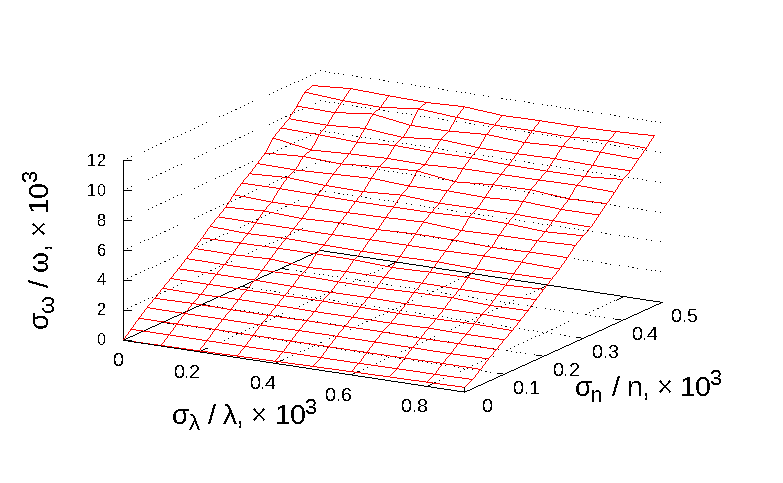
\includegraphics[scale=0.4]{figs/all/p2.txt_coeff0.dat.eps} & 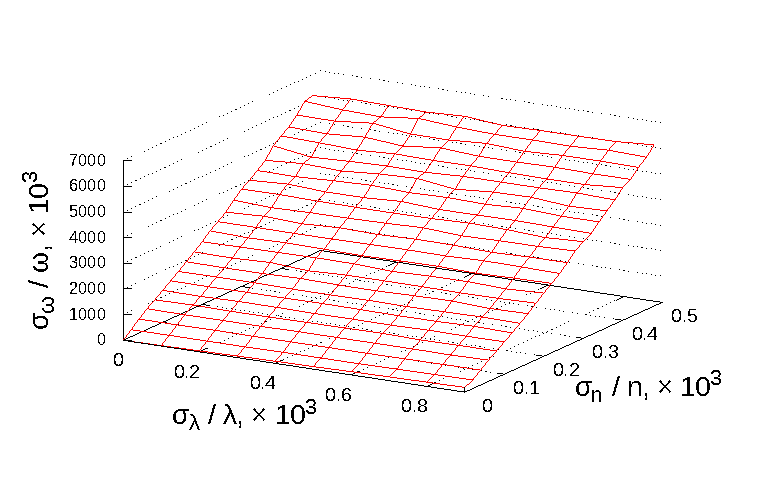
\includegraphics[scale=0.4]{figs/all/p2.txt_coeff1.dat.eps} & 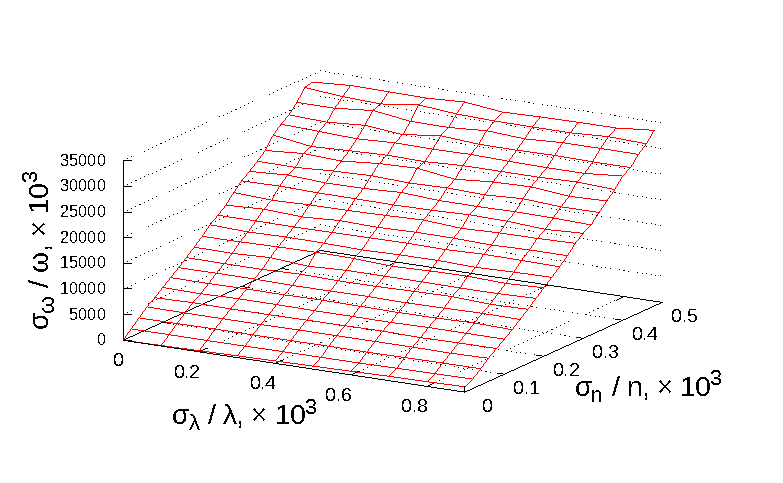
\includegraphics[scale=0.4]{figs/all/p2.txt_coeff2.dat.eps}
  \end{tabular}
  \label{tabl:res_incorrect}
\end{table}

Из графиков видно, что в случае формулы \eqref{eq:res_incorrect} дисперсия соответствующих
параметров существенно превышает таковую для \eqref{eq:res_0}. В частности, второй, третий
и четвертый коэффициенты имеют дисперсию, на порядки превышающую характерные значения самих
коэффициентов.

Данные результаты свидетельствуют о переобучении, и что полученная модель не может быть
использована для надежного приближения экспериментальных данных ввиду большой чувствительности
к шумам.

\begin{comment}
\paragraph{Исследование экспертного предположения.}

Экспертом предположено, что формула также может иметь вид
\begin{equation}
  n(\lambda) = a + \frac{b}{c - \frac{1}{\lambda^2}},
  \label{eq:resonance}
\end{equation}
если измерения находятся вблизи точки резонанса.

Результаты нахождения параметров $a, b$ и $c$ методом Левенберга-Марквардта
приведены в таблице \ref{tabl:resonance_coeffs}.

\begin{table}[h]
  \centering
  \footnotesize
  \begin{tabular}{| c | r | r | r | c |} \hline
	Материал	& $a$							& $b$					& $c$					& MSE						\\ \hline
	1			& $7.333 \cdot 10^{-3}$		& $3.509 \cdot 10^{-4}$	& $1.935 \cdot 10^{-4}$	& $1.7 \cdot 10^{-8}$		\\ \hline
	2			& $1.378$					& $2.352 \cdot 10^{-5}$	& $5.598 \cdot 10^{-5}$	& $3.6 \cdot 10^{-9}$		\\ \hline
  \end{tabular}
  \caption{Значения MSE и коэффициентов формулы \eqref{eq:resonance}.}
  \label{tabl:resonance_coeffs}
\end{table}

\begin{table}[h]
  \centering
  \footnotesize
  \begin{tabular}{l | c c c}
	  & Коэффициент 1 & Коэффициент 2 & Коэффициент 3 \\ \hline
	\begin{rotate}{90}Полимер 1\end{rotate} &	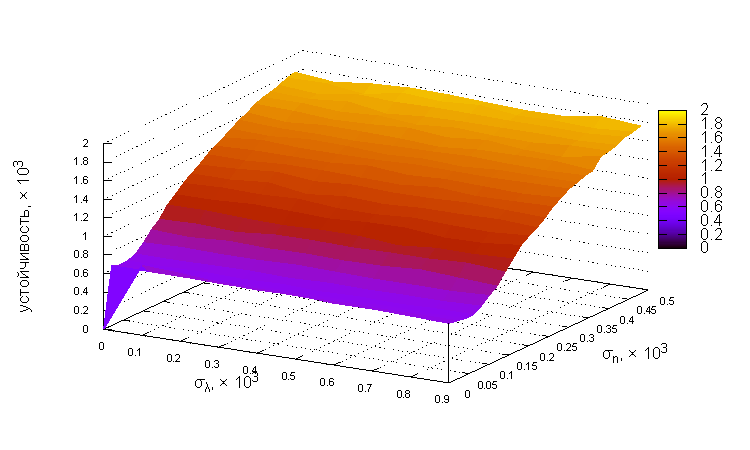
\includegraphics[scale=0.4]{figs/resonance/p1.txt_coeff0.dat.pdf} & 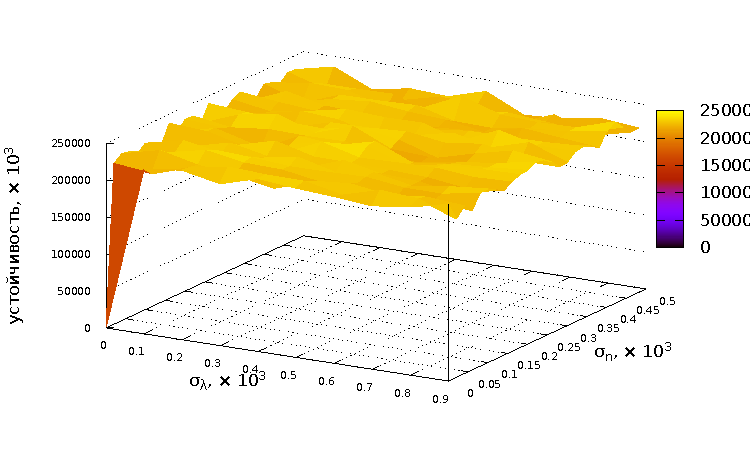
\includegraphics[scale=0.4]{figs/resonance/p1.txt_coeff1.dat.pdf} & 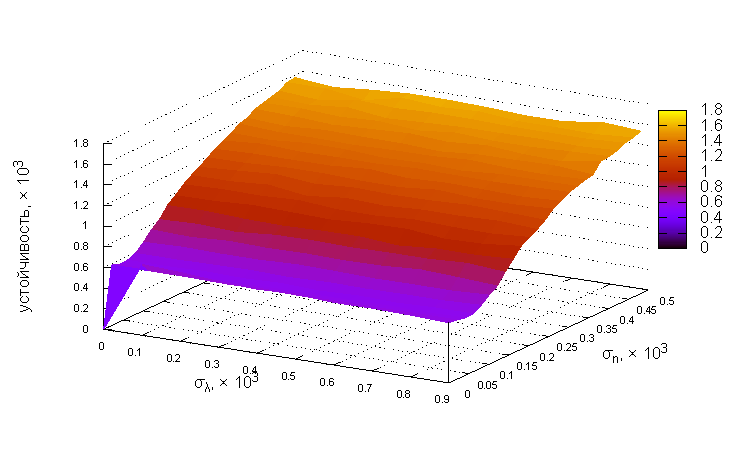
\includegraphics[scale=0.4]{figs/resonance/p1.txt_coeff2.dat.pdf} \\
	\begin{rotate}{90}Полимер 2\end{rotate} &	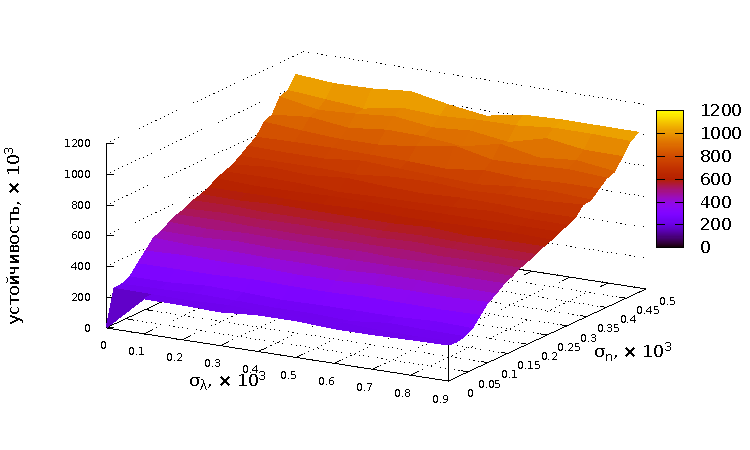
\includegraphics[scale=0.4]{figs/resonance/p2.txt_coeff0.dat.pdf} & 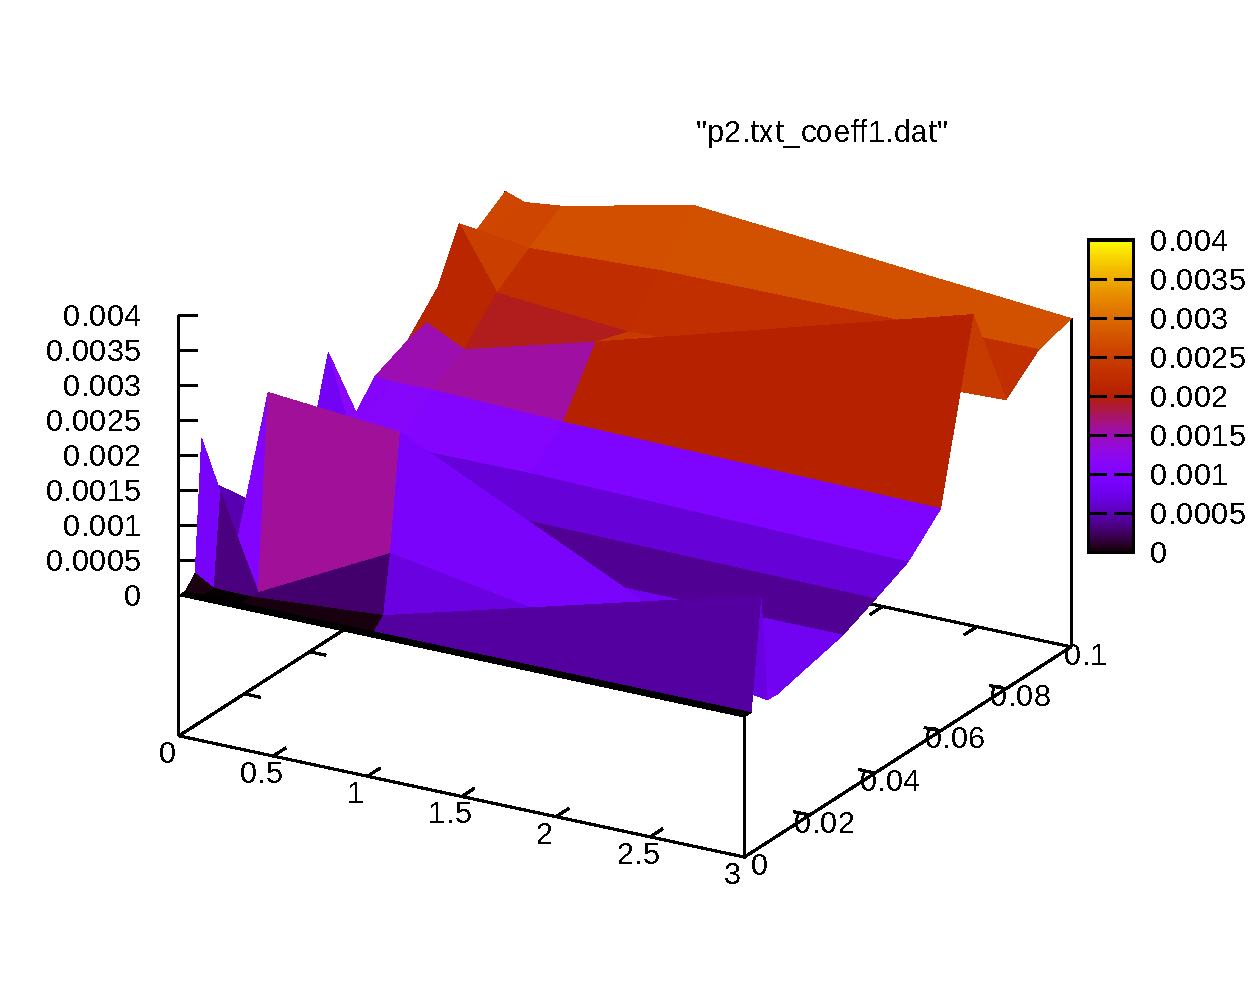
\includegraphics[scale=0.4]{figs/resonance/p2.txt_coeff1.dat.pdf} & 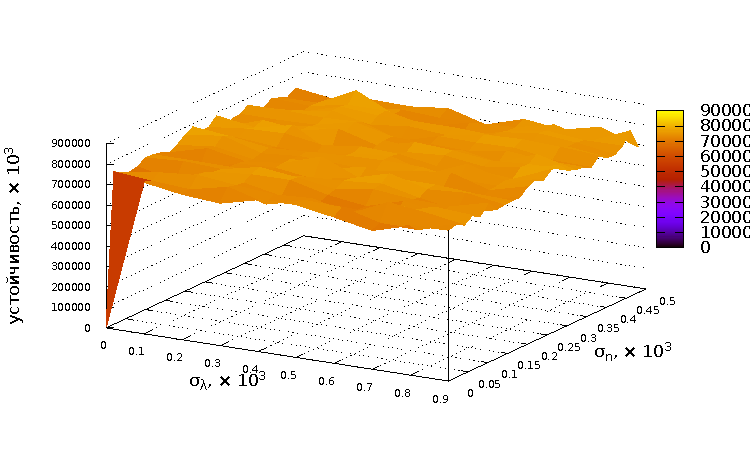
\includegraphics[scale=0.4]{figs/resonance/p2.txt_coeff2.dat.pdf}
  \end{tabular}
  \caption{Поверхности дисперсии для формулы \eqref{eq:resonance}.}
  \label{tabl:res_resonance}
\end{table}

Исследуем стабильность данного решения тем же методом, что и в
предыдущих случаях. Поверхности дисперсии приведены в таблице \ref{tabl:res_resonance}.

Отметим, что характерные дисперсия первого коэффициента на порядки больше, чем
для формулы \eqref{eq:res_0}, что затрудняет различение полимеров в смеси при
достаточно большой погрешности измерения $\lambda$. Кроме того, полученные значения
дисперсий коэффициентов позволяют говорить о, по-видимому, существенной неустойчивости
решения и, как следствие, невозможности его использования в качестве корректной модели.
Поверхности дисперсии также не являются настолько же гладкими, как для формулы
\eqref{eq:res_0}.

Все это позволяет заключить, что, хотя экспериментальные данные хорошо
описываются формулой \eqref{eq:resonance}, они не являются корректными с
экспертно-физической точки зрения.

\end{comment}

\section{Сходимость к классическому случаю}

Рассмотрим случай, когда зависимость линейна:
\[
  y = ax + b,
\]
и с учетом ошибок измерений представима в виде
\[
  y_i = ax_i + b + \xi_i \mid i \in \{ 1, \dots, n \},
\]
где ошибки $\xi_i$ независимы, $E(\xi_i) = 0; D(\xi_i) = \sigma^2$ \cite{Vatunin05}.
То есть, рассматривается случай независимости ошибки измерения от точки измерения,
при этом независимая переменная измеряется точно.

Перейдем к представлению
\[
  y_i = a(x_i - \overline{x}) + b + \xi_i \mid i \in \{ 1, \dots, n \},
\]
для которого, согласно \cite{Vatunin05}, случайные величины $a$ и $b$ независимы
и нормально распределены, и, кроме того, их дисперсии выражаются известными соотношениями:
\begin{equation}
  \label{eq:classic_da}
  D(a) = \frac{\sigma^2}{\sum_{i = 1}^n (x_i - \overline{x})^2}.
\end{equation}
\begin{equation}
  \label{eq:classic_db}
  D(b) = \frac{\sigma^2}{n}.
\end{equation}

Рассмотрим, насколько результаты предложенного метода отличаются от значений,
полученных согласно \eqref{eq:classic_da} и \eqref{eq:classic_db}. Для этого исследуем
зависимость относительной разности между этими значениями и эмпирическими значениями устойчивости от
числа итераций N:
\[
  \delta_1 = \frac{| \mathbf{T}^N_y(1) - D(a) |}{D(a)},
\]
\[
  \delta_2 = \frac{| \mathbf{T}^N_y(2) - D(b) |}{D(b)}.
\]

Соответствующие графики для функции $y = 2x + 1 + \xi_i$ на интервале $x \in [0; 10]$ при
$n = 10$ порождённых точках и $D(\xi_i) = 10$ приведены на фиг. \ref{fig:classic_var10_n10}.
В частности, на фиг. \ref{fig:classic_var10_n10_begin}
представлена начальная часть графика при количестве итераций $N$, меньшем $5 \cdot 10^5$, 
на фиг. \ref{fig:classic_var10_n10_middle}~--- средняя часть (при $N$ от $5 \cdot 10^5$
до $10^7$), а на фиг. \ref{fig:classic_var10_n10_end}~--- характер сходимости при больших $N$
(от $10^7$ до $10^8$).

Аналогичные графики приведены для $n = 10$ и $D(\xi_i) = 1$ и $n = 50$ и $D(\xi_i) = 1$
соответственно на фиг. \ref{fig:classic_var1_n10} и \ref{fig:classic_var1_n50}.

Из графиков видно, что значения разности стабилизируются в районе $(1.5 \div 3) \cdot 10^6$
итераций и не демонстрируют явной зависимости от числа точек или дисперсии погрешности.

\begin{figure}[h!]
  \begin{subfigure}[b]{0.3\textwidth}
    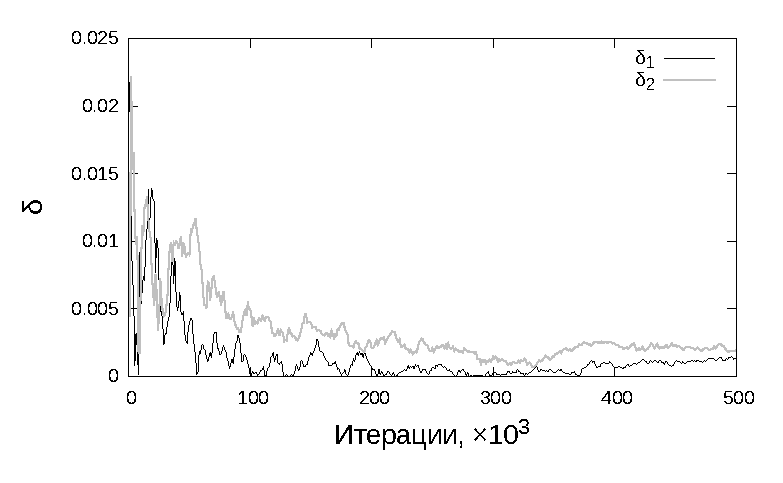
\includegraphics[width=\textwidth]{figs/classic/linear_log_1x_2_samples_10_variance_10_norm.log_0_500.eps}
    \caption{$N \in [0;~5 \cdot 10^5]$}
    \label{fig:classic_var10_n10_begin}
  \end{subfigure}
  \begin{subfigure}[b]{0.3\textwidth}
    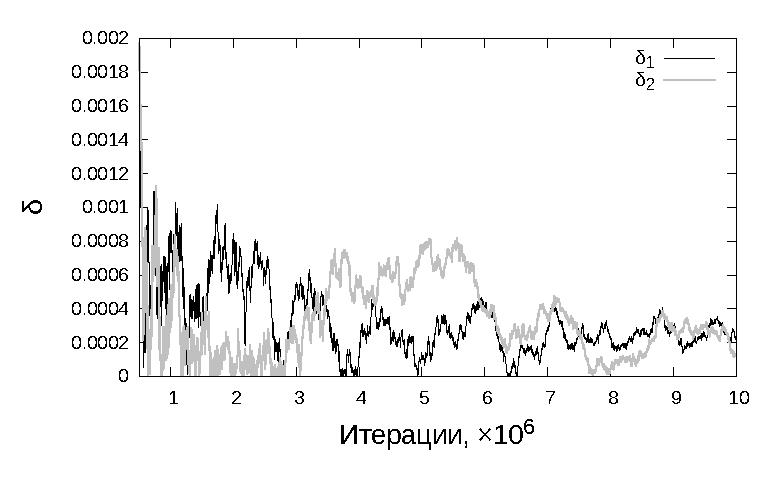
\includegraphics[width=\textwidth]{figs/classic/linear_log_1x_2_samples_10_variance_10_norm.log_500_10000.eps}
    \caption{$N \in [5 \cdot 10^5;~10^7]$}
    \label{fig:classic_var10_n10_middle}
  \end{subfigure}
  \begin{subfigure}[b]{0.3\textwidth}
    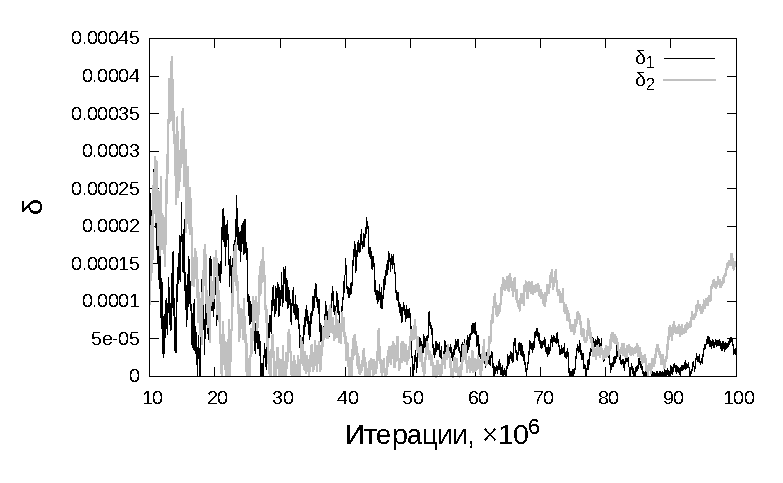
\includegraphics[width=\textwidth]{figs/classic/linear_log_1x_2_samples_10_variance_10_norm.log_end.eps}
    \caption{$N \in [10^7;~10^8]$}
    \label{fig:classic_var10_n10_end}
  \end{subfigure}
  \caption{Зависимость $\delta$ от числа итераций $N$ при $D(\xi) = 10$ и $n = 10$.}
  \label{fig:classic_var10_n10}
\end{figure}

\begin{figure}[h!]
  \begin{subfigure}[b]{0.3\textwidth}
    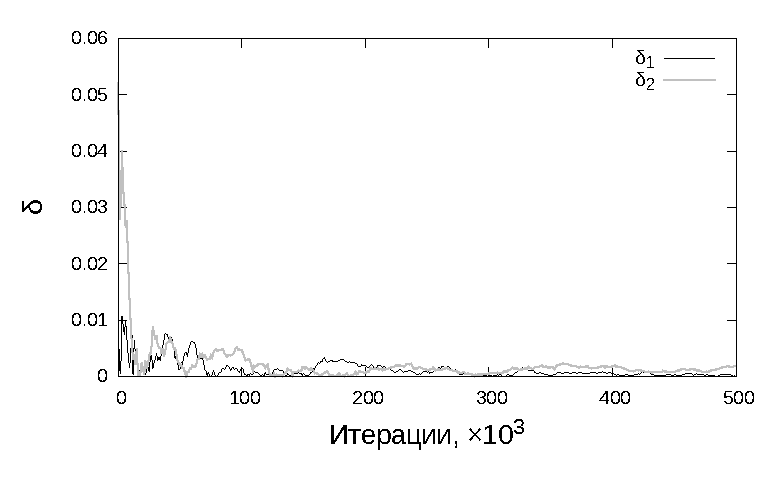
\includegraphics[width=\textwidth]{figs/classic/linear_log_1x_2_samples_10_variance_1_norm.log_0_500.eps}
    \caption{$N \in [0;~5 \cdot 10^5]$}
    \label{fig:classic_var1_n10_begin}
  \end{subfigure}
  \begin{subfigure}[b]{0.3\textwidth}
    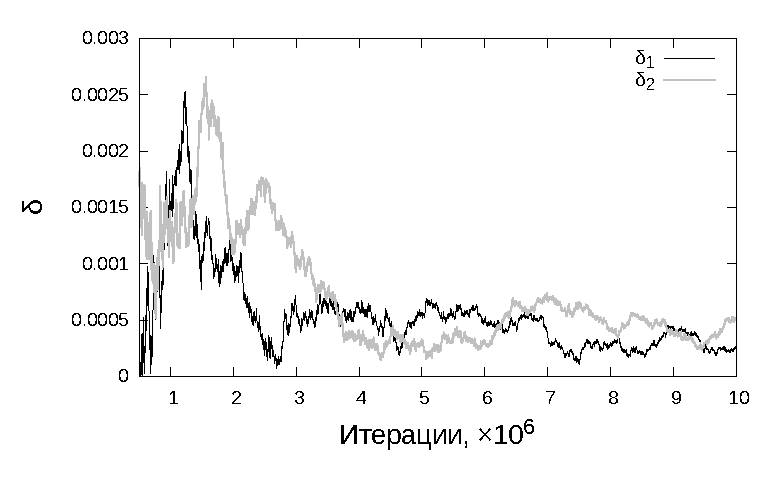
\includegraphics[width=\textwidth]{figs/classic/linear_log_1x_2_samples_10_variance_1_norm.log_500_10000.eps}
    \caption{$N \in [5 \cdot 10^5;~10^7]$}
    \label{fig:classic_var1_n10_middle}
  \end{subfigure}
  \begin{subfigure}[b]{0.3\textwidth}
    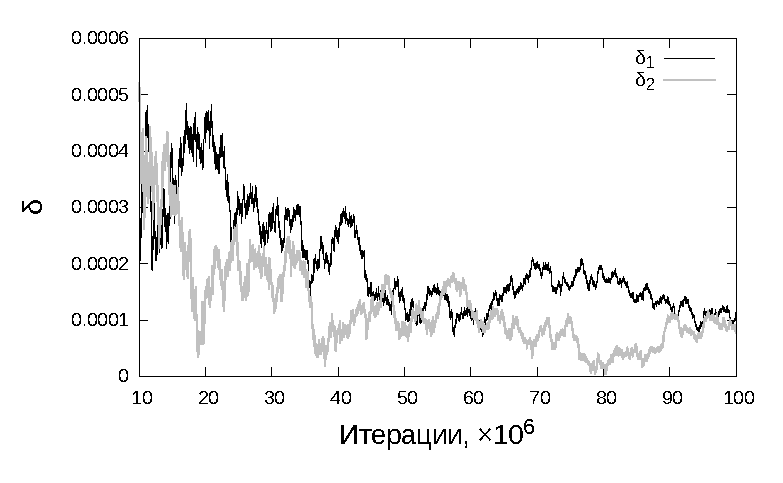
\includegraphics[width=\textwidth]{figs/classic/linear_log_1x_2_samples_10_variance_1_norm.log_end.eps}
    \caption{$N \in [10^7;~10^8]$}
    \label{fig:classic_var1_n10_end}
  \end{subfigure}
  \caption{Зависимость $\delta$ от числа итераций $N$ при $D(\xi) = 1$ и $n = 10$.}
  \label{fig:classic_var1_n10}
\end{figure}

\begin{figure}[h!]
  \begin{subfigure}[b]{0.3\textwidth}
    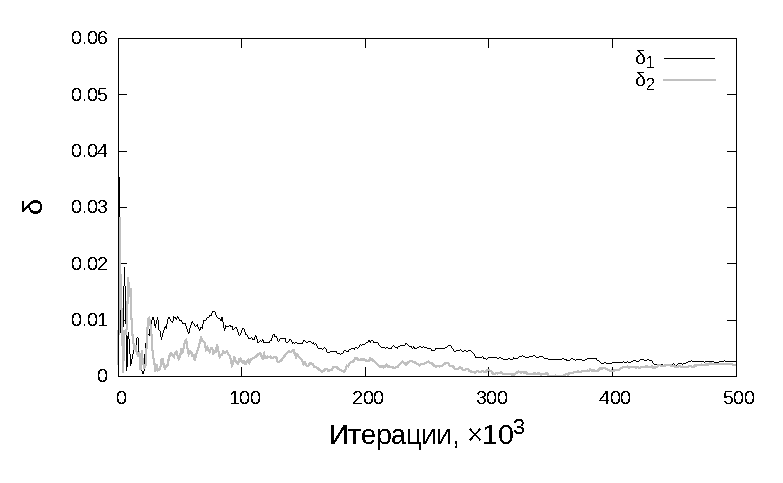
\includegraphics[width=\textwidth]{figs/classic/linear_log_1x_2_samples_50_variance_1_norm.log_0_500.eps}
    \caption{$N \in [0;~5 \cdot 10^5]$}
    \label{fig:classic_var1_n50_begin}
  \end{subfigure}
  \begin{subfigure}[b]{0.3\textwidth}
    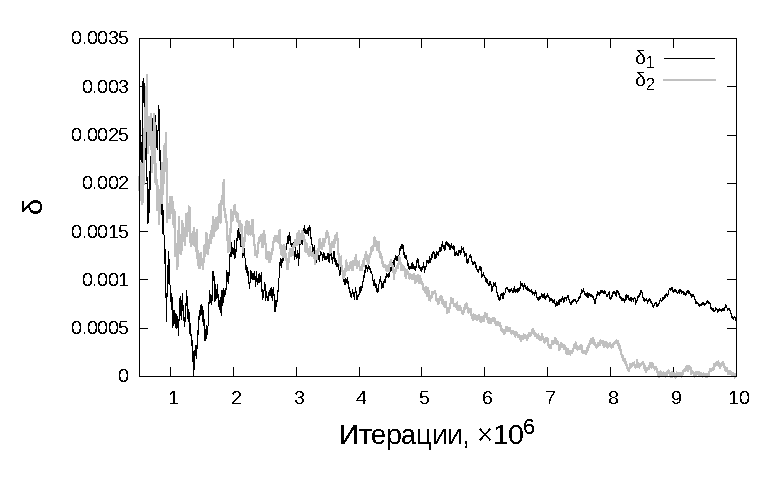
\includegraphics[width=\textwidth]{figs/classic/linear_log_1x_2_samples_50_variance_1_norm.log_500_10000.eps}
    \caption{$N \in [5 \cdot 10^5;~10^7]$}
    \label{fig:classic_var1_n50_middle}
  \end{subfigure}
  \begin{subfigure}[b]{0.3\textwidth}
    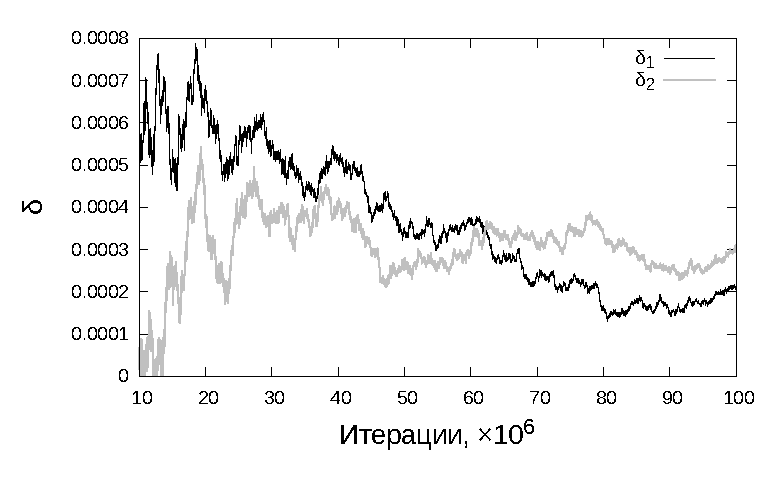
\includegraphics[width=\textwidth]{figs/classic/linear_log_1x_2_samples_50_variance_1_norm.log_end.eps}
    \caption{$N \in [10^7;~10^8]$}
    \label{fig:classic_var1_n50_end}
  \end{subfigure}
  \caption{Зависимость $\delta$ от числа итераций $N$ при $D(\xi) = 1$ и $n = 50$.}
  \label{fig:classic_var1_n50}
\end{figure}

\section{Заключение}

Предложенный в \cite{Rudoy13} алгоритм позволяет получить интерпретируемую аналитическую
формулу, описывающую зависимость коэффициента преломления среды от длины волны.
Введенный штраф за сложность позволяет избежать переобучения без использования методов
вроде скользящего контроля, и, таким образом, отпадает необходимость в контрольной выборке.

Хотя другие алгоритмы, такие как SVM-регрессия, могут демонстрировать более высокое
качество приближения данных, их результаты неинтерпретируемы и не защищены от переобучения
<<по построению>>, поэтому требуют разделения выборки на обучающую и контрольную. Кроме
того, их структурные параметры так же требуют оценки по методам вроде кросс-валидации.

Предложенный в настоящей работе метод оценки стабильности решения позволяет исследовать вклад различных
членов результирующей суперпозиции и зависимость изменения этих членов от
случайных шумов во входных данных. В частности, в прикладных областях данный метод позволяет
выявить, какие именно элементы признакового описания объектов в генеральной совокупности
наиболее чувствительны к шуму. Кроме того, для корректных с экспертной точки зрения
решений оказывается, что они стабильны, в то время как некорректные результаты нестабильны.

\FloatBarrier

\bibliographystyle{babunsrt-lf}
%\bibliographystyle{babunsrt}
%\bibliographystyle{unsrt}
\bibliography{bibliography}

\end{document}
